%%%%%%%%%%%%How does a GPS work and draw the state diagram for the GPS.Describe the different alternatives for measuring power consumption of a GPS%%%%%%%%%%%%%%%%%%%%%%%%%





\section{GPS}
The Global positioning system(GPS) is a space based radio navigation system developed by the Unites States Government, and has been operational since 1995.The system provides both timing and geolocation information to a GPS receiver anywhere on the Earth.  The system is not influenced by the number of receivers and can therefore serve an unlimited amount of users. The GPS system can deliver a position which is accurate within 22 meters horizontally if only one receiver is used. If multiple receivers is used positioning accuracy level of the order of a sub-centimeter to a few meters can be obtained \cite{GPS}. 

\subsection{Overview}
GPS consists three segments: space segment, control segment and the user segment. The space segment is a constellation of 24 satellites that are arranged so that  four to ten satellites is visible anywhere on the earth. Each satellite continuously broadcasts a signal composed of two carriers, two digital codes and a navigation message which contains the coordinates of the satellites as a function of the time. Each space vehicle as atomic clocks to ensure the integrity of the navigation message. The codes and the navigation message gets modulated with the two carrier frequencies.  \\If the distance between three satellites are known, the location of the receiver can be determined by measuring the angles with the respect of the each satellite.  GPS needs an additional satellite to account for the clock offset. Figure \ref{fig:GPS} shows the resection that is used by the satellites to determine the position.\\

\begin{minipage}[t]{0.8\textwidth}
\centering
    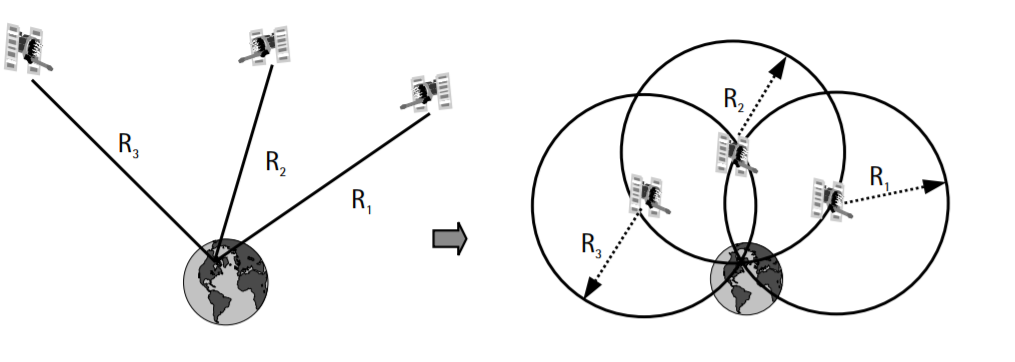
\includegraphics[width=0.8\textwidth]{Images/gps.PNG}\\
    \captionsetup{justification=centering}
    \captionof{figure}{Resection used by the satellites to determine the position}
    \label{fig:GPS}
\end{minipage}


  
  
  A method for determining the velocity of a GPS is by estimating the Doppler frequency of the received signal. The Doppler shift is caused by the relative motion of the receiver and the SV. The two carrier frequencies L1 and L2 that the satellites transmits are generated at 1.5 MHz and 1,2 MHz respectively.  Each SV transmits the L1 and L2 signal but the code modulation for each is different to avoid interference. The two digital code coarse acquisition code (C/A) and precision code(P) consists of a stream of binary digits. The codes are generated using an algorithm and enables a receiver to distinguish the satellites since each have their own set of codes. The navigation message contains the ephemeris, the almanac, the health of the SV, the clock correction, and the atmospheric data. 
  
  
  
  
  The satellites broadcasts two types of navigation messages the Almanac and the Ephemeris. The Almanac contains course date for all the Space Vechicles(SV). Each SV broadcast this for ALL SVs. The Almanac is valid for up to several months. The Ephemeris contains precise information about orbital position and clock correction is only valid for up to 30 minutes. Both of these are critical for getting a GPS fix, and they are often one of the time limiting factor for getting the position. 
  An outdated almanac or ephemeris can cause a slow start, this can happen if the receiver hasn't been used in a while, a cold start is done or the receiver has traveled a far distance while turned off.
  
  A GPS reciever is often in of two states: Its in 
